% !TeX document-id = {631e44a8-cd91-47da-bf82-1571f8787194}
% !TeX TXS-program:compile = txs:///pdflatex/[--shell-escape]

\documentclass{class/thesis}

\usepackage{pgfplots} 

%%%%%%%%%%%%%%%%%%%%%%%%%%%%%%%%%%%%%%%%%%%%%%%%%%%%%%%%%%%%
% Bitte ergänzen Sie Ihre persönlichen Daten innerhalb     %
% der im Folgenden inkludierten Datei properties.tex       %
%%%%%%%%%%%%%%%%%%%%%%%%%%%%%%%%%%%%%%%%%%%%%%%%%%%%%%%%%%%%

%%%%%%%%%%%%%%%%%%%%%%%%%%%%%%%%%%%%%%%%%%%%%%%%
% Titel der Arbeit                             %
%%%%%%%%%%%%%%%%%%%%%%%%%%%%%%%%%%%%%%%%%%%%%%%%
\thesistitle{Entwicklung eines Log-strukturierten Heaps für NVRAM}

%%%%%%%%%%%%%%%%%%%%%%%%%%%%%%%%%%%%%%%%%%%%%%%%
% Schlüsselwörter                              %
%%%%%%%%%%%%%%%%%%%%%%%%%%%%%%%%%%%%%%%%%%%%%%%%
\thesiskeywords{NVRAM, Log-strukturiert, Log-Struktur, Heap}

%%%%%%%%%%%%%%%%%%%%%%%%%%%%%%%%%%%%%%%%%%%%%%%%
% Sprache der Arbeit                           %
%                                              %
%   ngerman  - Deutsch (neue Rechtschreibung)  %
%   english  - Englisch                        %
%%%%%%%%%%%%%%%%%%%%%%%%%%%%%%%%%%%%%%%%%%%%%%%%
\thesislanguage{ngerman}

%%%%%%%%%%%%%%%%%%%%%%%%%%%%%%%%%%%%%%%%%%%%%%%%
% Art der Arbeit                               %
%                                              %
%   bachelor  - Bachelorarbeit                 %
%   master    - Masterarbeit                   %
%   project   - Projektarbeit                  %
%%%%%%%%%%%%%%%%%%%%%%%%%%%%%%%%%%%%%%%%%%%%%%%%
\thesistype{bachelor}

%%%%%%%%%%%%%%%%%%%%%%%%%%%%%%%%%%%%%%%%%%%%%%%%
% Ausgabe von Verzeichnissen                   %
%                                              %
%   true   - Aktiviert                         %
%   false  - Deaktiviert                       %
%%%%%%%%%%%%%%%%%%%%%%%%%%%%%%%%%%%%%%%%%%%%%%%%
\listofalgorithmsenabled{true}
\listoffiguresenabled{true}
\listoftablesenabled{true}

%%%%%%%%%%%%%%%%%%%%%%%%%%%%%%%%%%%%%%%%%%%%%%%%
% Vollständiger Name                           %
%%%%%%%%%%%%%%%%%%%%%%%%%%%%%%%%%%%%%%%%%%%%%%%%
\thesisauthor{Maximilian Vogel}

%%%%%%%%%%%%%%%%%%%%%%%%%%%%%%%%%%%%%%%%%%%%%%%%
% Geburtsort                                   %
%%%%%%%%%%%%%%%%%%%%%%%%%%%%%%%%%%%%%%%%%%%%%%%%
\authorbirthplace{Wuppertal}

%%%%%%%%%%%%%%%%%%%%%%%%%%%%%%%%%%%%%%%%%%%%%%%%
% Datum der Abgabe                             %
%%%%%%%%%%%%%%%%%%%%%%%%%%%%%%%%%%%%%%%%%%%%%%%%
\submissiondate{21. September 2023}

%%%%%%%%%%%%%%%%%%%%%%%%%%%%%%%%%%%%%%%%%%%%%%%%
% Erstgutachter                                %
%%%%%%%%%%%%%%%%%%%%%%%%%%%%%%%%%%%%%%%%%%%%%%%%
\firstreviewer{Prof. Dr. Michael Schöttner}

%%%%%%%%%%%%%%%%%%%%%%%%%%%%%%%%%%%%%%%%%%%%%%%%
% Zweitgutachter                               %
%%%%%%%%%%%%%%%%%%%%%%%%%%%%%%%%%%%%%%%%%%%%%%%%
\secondreviewer{Prof. Dr. Stefan Conrad}

%%%%%%%%%%%%%%%%%%%%%%%%%%%%%%%%%%%%%%%%%%%%%%%%
% Betreuer                                     %
%%%%%%%%%%%%%%%%%%%%%%%%%%%%%%%%%%%%%%%%%%%%%%%%
\supervisor{Prof. Dr. Michael Schöttner}

\begin{document}

  \begin{thesis}

    %%%%%%%%%%%%%%%%%%%%%%%%%%%%%%%%%%%%%%%%%%%%%%%%%%%%%%%%%%%%%%%%%
    % Die folgenden Kapitel dienen lediglich als Hilfestellung      %
    % und müssen somit mit der Fertigstellung des finalen Dokuments %
    % unbedingt entfernt werden.                                    %
    %%%%%%%%%%%%%%%%%%%%%%%%%%%%%%%%%%%%%%%%%%%%%%%%%%%%%%%%%%%%%%%%%

%    \include{chap/einleitung}
%    \include{chap/gliederung}
%    \include{chap/struktur}
%    \include{chap/organisation}
%    \include{chap/text}
%    \include{chap/zitieren}
%    \include{chap/auflistungen}
%    \include{chap/bilder}
%    \include{chap/tabellen}
%    \include{chap/matheumgebung}
%    \include{chap/code}

	\chapter{Einleitung}
	
	NVRAM ist eine neue Art von Speicher, welche die Vorteile von DRAM und SSDs vereint, wobei die Geschwindigkeit und Persistenz zu den wichtigsten gehören. 
	Programme zu entwickeln, die NVRAM benutzten, funktioniert ähnlich wie welche die es nicht tun, jedoch gibt es einige Dinge zu beachten.
	Da NVRAM, im Gegensatz zu DRAM, persistent ist, muss darauf geachtet werden, dass auch nach einem Absturz die Daten konsistent sind. Bzw. wenn sie es nicht, muss ein konsistenter Zustand wiederhergestellt werden.
	Das PMDK \cite{PMDK:Docs} stellt mehrere Bibliotheken zur Verfügung, die einem das Entwickeln für NVRAM erleichtern. Eine dieser Bibliotheken wird auch in dieser Arbeit genutzt.
	
	Das Ziel dieser Arbeit ist es einen Log-strukturierten Heap für NVRAM zu entwickeln, bei diesem werden allozierte Daten einfach immer am Ende angehangen. 
	Bestehende Daten dürfen allerdings nicht verändert werden, sodass sie bei einer Aktualisierung neu eingefügt werden müssen. 
	Um freigegebenen Speicher wiederverwenden zu können, wird das Log von einem Cleaner kompaktiert und aufgeräumt.
	So wird eine Fragmentierung des Speichers vermieden, welche z.B. bei general-purpose Allokatoren, wie sie auch meist für DRAM verwendet werden, vorkommt und bei NVRAM noch schwerwiegender ist.
	
	Die Implementierung wird mit Hilfe von pmemids\_bench \cite{Bench:Git} evaluiert und mit einem DRAM Allokator, sowie einem general-purpose Allokator für NVRAM verglichen.
	Die Ergebnisse zeigen, dass die Stärke der Log-Struktur eine deutlich schnellere Allokation von Daten ist, jedoch langsamer Daten gelesen und aktualisiert werden können.
	
	
	

	\chapter{Grundlagen}
	
	\section{NVRAM}
	NVRAM ist die Abkürzung für \glqq{}Non Volatile Random Access Memory\grqq{}, also nicht flüchtiger Hauptspeicher. Eine andere häufig genutzte Bezeichnung ist \glqq{}Persistent Memory\grqq{}.
	Wie in Abbildung \ref{bildSpeicherHierarchie} zu sehen ist, ordnet sich NVRAM in der Speicher Hierarchie zwischen DRAM und SSDs ein und vereint somit die Vorteile von DRAM und Sekundärspeicher.
	
	\begin{figure}[h]
		\centering
		\begin{subfigure}[b]{1.0\textwidth}
			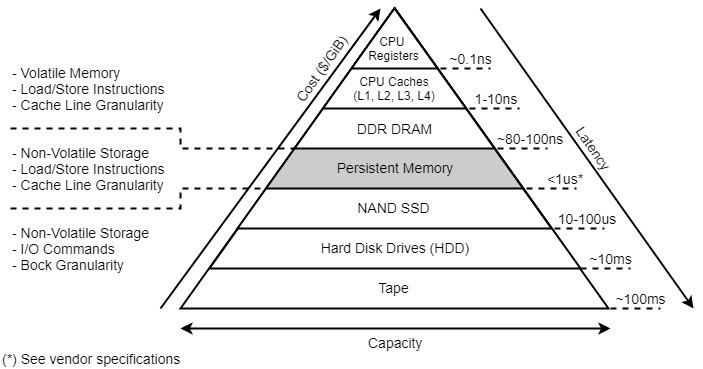
\includegraphics[width=1.0\linewidth]{img/pmem_storage_pyramid}
		\end{subfigure}
		\caption{Speicher Hierarchie \cite{PMEM.IO:Introduction}}
		\label{bildSpeicherHierarchie}
	\end{figure}
	
	NVRAM ist im Gegensatz zu DRAM, wie der Name schon sagt, persistent. Somit bleiben die Daten im Speicher erhalten, wenn der Computer, sei es bewusst oder z.B. durch einen Stromausfall, ausgeschaltet wird und sind  nach dem Systemstart direkt wieder nutzbar, ohne dass sie erst vom Sekundärspeicher geladen werden müssen \cite{Scargall:2020:PPM}.
	Die Geschwindigkeit von NVRAM kommt zwar nicht ganz an die von DRAM heran, ist aber trotzdem um ein vielfaches schneller, als die von SSDs \cite{PMEM.IO:Introduction}.
	Die Speicherkapazität und der Preis ordnen sich ebenfalls entsprechend zwischen DRAM und SSDs ein \cite{PMEM.IO:Introduction} und die Lebensdauer von NVRAM ist länger, als die von SSDs \cite{Scargall:2020:PPM}. \\
	Außerdem ist NVRAM Byte adressierbar und es können per \glqq{}Direct Access\grqq{}(DAX) direkt Load und Store Instruktionen ausgeführt werden, ohne Code aus dem Kernel zu verwenden \cite{Rudoff:2017:PMP}. 
	Das bringt folgenden Vorteil: Angenommen man möchte 8 Byte in seinen Daten ändern, dann kann man, wenn die Daten im NVRAM liegen, diese 8 Byte direkt schreiben. Wenn die Daten jedoch im Sekundärspeicher liegen, muss erst der entsprechende Block geladen werden, dieser ist meist 4 KB groß. Dann können die Daten aktualisiert werden und anschließend muss der Block wieder in den Sekundärspeicher geschrieben werden \cite{Scargall:2020:PPM}. \\
	Da NVRAM persistent ist, müssen die Daten im Speicher wiedergefunden werden können und können nicht wie bei DRAM anonym sein. Um das zu erreichen, wird dieselbe Semantik, wie bei Dateien im Sekundärspeicher verwendet. Die Daten werden mit den Standardbefehlen gemappt und haben einen Namen, sowie Zugriffsrechte. Nachdem sie gemappt wurden, kann per DAX auf sie zugegriffen werden \cite{Rudoff:2017:PMP}. Es ist wichtig zu beachten, dass es nicht alleine ausreicht Daten per Store Instruktion zu schreiben, sondern man auch die Caches flushen muss, andernfalls sind sie nicht persistiert und könnten verloren gehen \cite{Rudoff:2017:PMP}.
	Die Reihenfolge in der die Daten, dann persistiert werden ist aber nicht zwingend die selbe, in der sie auch geschrieben wurden.
	Außerdem können nur 8 Byte atomar geschrieben werden, somit muss bei größeren Flushes darauf geachtet werden die Daten im Falle eines Absturzes konsistent zu halten \cite{PMEM.IO:Introduction}.
%	\todo[inline]{Reihenfolge und (8 Byte Atomarität bei Stromausfall)}
	
	
	
	\section{Persistent Memory Development Kit}
	
	Das Persistent Memory Development Kit, kurz PMDK, ist eine Sammlung von Intel entwickelter Open Source Bibliotheken, welche Funktionen zur einfacheren Nutzung von NVRAM zur Verfügung stellen \cite{Scargall:2020:PPM}.
	Es enthält die folgenden Bibliotheken.
	
	\textbf{libpmem} bietet low-level Unterstützng für NVRAM und erkennt automatisch die vorhandenen Funktionen des Systems zum optimalen flushen und persistieren \cite{Scargall:2020:PPM}.
	
	\textbf{libpmem2} ist eine neue Version von libpmem und bietet ein allgemeineres und plattformunabhängiges Interface \cite{PMDK:Docs}.

	\textbf{libpmemobj} bietet unter anderem einen general-purpose Allokator und Transaktionen. Sie ist die Bibliothek, welche einem am meisten Arbeit abnimmt und für die meisten Fälle die einfachste Lösung \cite{PMDK:Docs}\cite{Scargall:2020:PPM}.
	
	\textbf{libpmempool} dient zur Verwaltung von Speicherpools im Sinne von libpmemobj \cite{PMDK:Docs}.
	\\
	\\
	Das PMDK enthält noch einige andere Bibliotheken, diese werden jedoch nicht mehr weiter entwickelt und erhalten keinen offiziellen Support mehr, daher werden sie hier nicht weiter erwähnt \cite{PMDK:Docs}.	

	
	\subsection{libpmem2}
	
	Da das Ziel dieser Arbeit ist, selbst Speicher zu allozieren, um eine Log-Struktur zu erreichen, kann libpmemobj nicht genutzt werden. Es wird also ausschließlich die Bibliothek libpmem2 benutzt, welche nur die grundlegenden Funktionen zum persistieren bereitstellt. Im folgenden werden diese anhand eines einfachen Beispiels erklärt. \\
	Zuerst muss die Datei geöffnet werden, in welcher die zu persistierenden Daten gespeichert werden sollen. Das geschieht wie im Codebeispiel in Zeile 8 zu sehen ist, genau so wie für normale Dateien im Dateisystem.
	Anschließend wird mit \code{pmem2\_config\_new} ein config struct erstellt, das für das Mapping des Speichers benötigt wird. Dort kann z.B. die Länge des Mappings gesetzt werden. Als einziges muss jedoch die Granularität gesetzt werden, dafür wird die Funktion \code{pmem2\_config\_set\_required\_store\_granularity} genutzt. Sie gibt die höchste Unterstützte Granularität der \glqq{}power-fail protected domain\grqq{} an, bei welcher das Programm noch läuft. Wenn \code{PMEM2\_GRANULARITY\_PAGE} angegeben wird, läuft das Programm also auch auf SSDs und nicht nur auf NVRAM.
	Um ein Mapping zu erstellen wird außerdem ein source struct benötigt, welches man mit der Funktion \code{pmem2\_source\_from\_fd} erhält. Mit Hilfe dieser beiden stucts und \code{pmem2\_map\_new} kann nun das Mapping, wie in Zeile 28, erstellt werden.
	
	\begin{codeblock}{libpmem2\_beispiel.c}{C}
		\begin{ccode}\\
			char *path = "/pmem/pmem_file";
			int fd;
			struct pmem2_config *cfg;
			struct pmem2_map *map;
			struct pmem2_source *src;
			pmem2_persist_fn persist;
			
			if ((fd = open(path, O_RDWR)) < 0) {
			    perror("open");
			    exit(1);
			}
			
			if (pmem2_config_new(&cfg)) {
			    pmem2_perror("pmem2_config_new");
			    exit(1);
			}
			
			if (pmem2_config_set_required_store_granularity(cfg, PMEM2_GRANULARITY_PAGE)) {
			    pmem2_perror("pmem2_config_set_required_store_granularity");
			    exit(1);
			}
			
			if (pmem2_source_from_fd(&src, fd)) {
			    pmem2_perror("pmem2_source_from_fd");
			    exit(1);
			}
			
			if (pmem2_map_new(&map, cfg, src)) {
			    pmem2_perror("pmem2_map_new");
			    exit(1);
			}
		\end{ccode}
	\end{codeblock}
	
	Durch die Funktion \code{pmem2\_map\_get\_address} erhält man die Adresse des gemappten Speichers, um auch auf ihm arbeiten zu können. Das ist jetzt nach dem selben Prinzip möglich, wie man es gewohnt ist.
	Es können also einfach Funktionen wie \code{strcpy} aufgerufen werden, um einen String an die gewünschte Speicheradresse zu schreiben.
	Dieser wird jedoch dadurch noch nicht garantiert persistiert. Dafür muss man zuerst \code{pmem2\_get\_persist\_fn} aufrufen, welche eine Funktion zum persistieren zurückgibt. Der zurückgegebenen Funktion übergibt man dann die Startadresse und die Länge des zu persistierenden Bereichs.
	Am Ende des Programms muss, wie bei allozierten und geöffneten Ressourcen üblich, alles wieder freigegeben und geschlossen werden, um Speicherlecks zu verhindern.
	
	\begin{codeblock}{libpmem2\_beispiel.c}{C}
		\begin{ccode}\\			
			char *addr = pmem2_map_get_address(map);
			
			strcpy(addr, "hello, persistent memory");
			
			persist = pmem2_get_persist_fn(map);
			persist(addr, size);
			
			pmem2_unmap(&map);
			pmem2_source_delete(&src);
			pmem2_config_delete(&cfg);
			close(fd);
		\end{ccode}
	\end{codeblock}



	\section{Gründe für eine Log-Struktur}
	
	Ein Problem in der Speicherverwaltung ist die Fragmentierung des Speichers, wodurch Speicherplatz \glqq{}verloren\grqq{} geht, indem er nicht mehr genutzt werden kann. Dabei unterscheidet man zwischen zwei Fällen.
	Bei der internen Fragmentierung verbrauchen allozierte Daten nicht nur ihre tatsächliche Größe, sondern ein vielfaches der kleinstmöglichen Speicherblockgröße im System. Wenn ein System z.b. 32 Byte große Speicherblöcke hat und 33 Byte Speicherplatz alloziert werden sollen, werden trotzdem 64 Byte alloziert und es entsteht somit ein Speicherverschnitt von 31 Byte, welcher nicht genutzt werden kann.
	Externe Fragmentierung tritt auf, wenn Speicherplatz freigegeben wird. Dabei entstehen Lücken im Speicher, welche zwar genutzt werden können, allerdings nur von Daten, die auch in die Lücke hinein passen. Wenn es also viele kleine freie Stellen im Speicher gibt, ist zwar noch einiges an freiem Speicherplatz vorhanden, dieser ist aber praktisch nicht nutzbar, sofern die zu speichernden Daten nicht klein genug sind, um hineinzupassen.\\
	Allokatoren, die im Stil von DRAM an beliebigen Stellen Speicher allozieren können, können eine Speicherfragmentierung von über 50\% erreichen \cite{Rumble:FAST14}. Das stellt für NVRAM ein besonders großes Problem dar, da die Fragmentierung im Gegensatz zu DRAM auch über den Systemneustart hinaus erhalten bleibt.
	Log-strukturierter Speicher verhindert interne Fragmentierung durch das einfache Anhängen der Daten an das Ende des Logs. Und externe Fragmentierung durch das Kompaktieren des Speichers durch den Cleaner \cite{HU:ATC17}. 
	Dadurch kann Log-strukturierter Speicher eine Speicherauslastung von 80-90\% erreichen, ohne dabei Einbuße der Performance zu haben \cite{Rumble:FAST14}. 
	
	
	\subsection{Beispiele für Log-strukturierten Speicher}
	
	Bekannte Beispiele für Log-strukturierten Speicher sind Sprite LFS \cite{Rosenblum:1992} und RAMCloud \cite{Rumble:FAST14}. Sprite LFS ist die erste Implementierung eines Log-strukturierten Dateisystems und RAMCloud implementiert Log-strukturierten DRAM mit Backups auf mehreren Servern.
	Diese Arbeit orientiert sich an den beiden genannten Beispielen, implementiert die Log-Struktur jedoch auf NVRAM und nicht auf DRAM oder sekundär Speicher.
	Eine Erklärung was Log-strukturierter Speicher genau ist, befindet sich in Abschnitt \ref{Log-struktur_Erklärung}.

	


	\chapter{Konzept}	
	
	\section{Prinzip eines Log-strukturierten Speichers} \label{Log-struktur_Erklärung}
	
	Hinweis: Die Informationen zu diesem Abschnitt stammen aus \cite{Rosenblum:1992}, \cite{Rumble:FAST14} und \cite{HU:ATC17}. Das Prinzip ist nach eigenem Verständnis nach dem Lesen dieser Quellen wiedergegeben worden.
	\\
	\\
	In einem Log-strukturierten Speicher werden neue Daten einfach an das Ende des Logs angehangen, dadurch spart man sich die Zeit zuerst eine passende Stelle finden zu müssen. Klassisch strukturierte Speicher benutzten zwar auch Logs, allerdings werden die Daten dort nur temporär gespeichert und anschließend an den richtigen Speicherplatz geschrieben. Die Daten müssen also, im Gegensatz zu Log-strukturiertem Speicher, zwei mal geschrieben werden, bevor sie persistiert sind.
	Da das Log unveränderlich ist können Daten in ihm nicht aktualisiert werden, das hat die Folge, dass aktualisierte Daten neu an das Log angehangen werden müssen. Alte Versionen der Daten müssen also entfernt werden, um keinen Speicherplatz zu verschwenden. Die durch das Löschen der Daten entstehenden Lücken können allerdings nicht genutzt werden, da neue Daten immer nur am Ende des Logs eingefügt werden.
	Dieses Problem löst der Cleaner. \\
	Der Cleaner hat zwei Aufgaben. Die erste ist das Löschen von Daten und das Finden veralteter Versionen inklusive anschließendem Löschen. Die zweite ist das Kompaktieren des Logs, wodurch freie Stellen im Log wieder benutzt werden können. \\
	In der Regel wird das Log in Segmente unterteilt. Wenn ein Segment mit Daten vollgeschrieben wurde, wird das nächste beschrieben. Der Cleaner kompaktiert das Log, indem er die Segmente durchgeht und noch aktuelle Daten in ein neues leeres Segment kopiert und dieses wieder in das Log einfügt. Das gesäuberte Segment steht jetzt wieder für neue Daten zur Verfügung. \\
	Welche Segmente der Cleaner zum kompaktieren auswählt und wie er die noch aktuellen Daten sortiert und wieder in das Log einfügt ist eine Frage der Implementierung und kann starke Auswirkungen auf die gesamte Performance haben.
	
	
	
	\section{Komponenten}
	Die Implementierung dieser Arbeit besteht aus drei Komponenten. Dem Log selbst, einer Hashtabelle und dem Cleaner. Das Log befindet sich in der gemappten Datei und besteht aus vielen aneinander gereihten Segmenten.
	Diese Segmente werden in mehreren Listen verwaltet, abhängig vom aktuellen Zustand des Segments. Es ist entweder leer und kann für neu allozierte Daten verwendet werden, wurde bereits befüllt und enthält eine beliebige Anzahl noch aktiver Daten, wird gerade mit neuen Daten beschrieben, wird vom Cleaner verwendet, um noch aktive Daten dort hinein zu kopieren oder ist eine Notfallsegment für den Cleaner. Diese Listen kann ein Segment nicht nach belieben wechseln, sondern nur nach den in Abbildung \ref{segmenteListenWechsel} zu sehenden Übergängen. Wann genau welche Wechsel stattfinden wird in Kapitel \ref{Implementierung} erläutert.
	
	\begin{figure}[h]
		\centering
		\begin{subfigure}[b]{1.0\textwidth}
			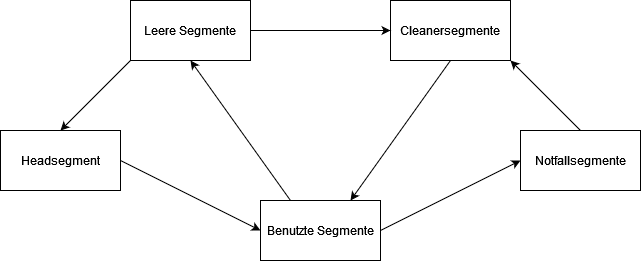
\includegraphics[width=1.0\linewidth]{img/SegmenteListenWechsel.drawio.png}
		\end{subfigure}
		\caption{Mögliche Wechsel  zwischen den Segmentlisten}
		\label{segmenteListenWechsel}
	\end{figure}
	
	Da sich die Position der Daten jeder Zeit ändern kann, wird bei der Allokation nicht die Adresse zurückgegeben, so wie man es auch von \code{malloc} kennt, sondern eine ID um die allozierten Daten im Log zu identifizieren.
	Diese ID wird zusammen mit der aktuellen Adresse der Daten als Key-Value-Paar in einer Hashtabelle gespeichert. Die Hashtabelle befindet sich im DRAM, um schnellere Zugriffe darauf zu haben. Am Ende des Programms werden diese Daten persistiert, damit sie beim nächsten Programmstart wieder nutzbar sind. \\
	Der Cleaner iteriert über die Benutzten Segmente und prüft, ob ein Segment gesäubert werden muss. Wenn das der Fall ist, geht er die Einträge des Segments durch und kopiert die aktiven Daten in sein Cleanersegment. Das gesäuberte Segment kann jetzt wieder für neue Daten genutzt werden. Sobald sein Cleanersegment voll ist, wird es in die Liste der Benutzten Segmente eingefügt.
	

	
	
	\chapter{Implementierung} \label{Implementierung}
	
	\section{Offsets}
	
	Da der Speicher bei jedem Programmstart an eine andere Adresse gemappt wird, können keine Adressen gespeichert werden, um das Log zu verwalten. Daher werden alle Adressen, die gespeichert werden müssen in Offsets konvertiert, diese geben den Abstand zum Beginn des gemappten Speichers an. Um dann auf die Daten am Offset zugreifen zu können, kann er einfach wieder zu einer Adresse konvertiert werden. 
	Dafür wurden die beiden Funktionen \code{offset\_to\_pointer} und \code{pointer\_to\_offset} implementiert. Offsets werden durch den Typ \code{pmo\_t} repräsentiert, welcher ein \code{uintptr\_t} und somit je nach System ein \code{unsigned long int} oder \code{unsigned int} ist.
	
	
	
	\section{Metadaten}
	
	Allozierte Daten werden in einem Logeintrag gespeichert, dieser ist definiert durch den Typ \code{log\_entry\_t}. Neben den allozierten Daten beinhaltet dieser die ID des Eintrags, die Versionsnummer, welche bei jeder Aktualisierung inkrementiert wird, die Länge der reinen Daten, also ohne die Länge der Metadaten, und ein Flag, welches angibt, ob der Eintrag vom Cleaner gelöscht werden kann.
	
	Die Logeinträge werden in den Segmenten abgelegt, welche durch den Typ \code{segment\_t} definiert sind. Sie beinhalten ebenfalls eine ID und speichern den bereits belegten Speicherplatz des Segments, außerdem halten sie den Offset des nächsten Segments der entsprechenden Segmentliste. Wenn das Segment das letzte einer Liste ist, ist der Offset des nächsten Segments \code{NULL}.
	Die Segmentlänge ist per Define in der Datei \code{log\_pmem\_types.h} gesetzt und beträgt 4 KiB, also 4096 Byte. Diese Länge beinhaltet den benötigten Platz für die Metadaten. Der tatsächlich für Logenträge verwendbare Platz beträgt 4072 Byte, da \code{segment\_t} 24 Byte groß ist.
	
	Am Anfang des gemappten Speichers befinden sich die für das gesamte Log relevanten Metadaten, welche persistiert werden müssen und nicht im RAM liegen können, diese werden im struct \code{log\_t} gespeichert. Hier werden die Offsets des ersten und letzten Segments der Listen der freien Segmente, belegten Segmente, Cleanersegmente und Notfallsegmente gespeichert, außerdem wird hier der Offset des Headsegments gespeichert. 
	Für die Allokation relevant, ist die Position des Headsegments, an der als nächstes die neuen Daten geschrieben werden können. Hier könnte man zuerst denken, dass man dafür die Variable \code{used\_space} aus \code{segment\_t} verwenden kann, welche den bereits belegten Platz angibt.
	Das wird jedoch zum Problem, wenn ein Logeintrag freigegeben wird, der sich im Headsegment befindet. Dann würden nämlich bei der nächsten Allokation die zuletzt allozierten Daten einfach überschrieben werden. Die Position muss also separat gespeichert werden. Und da sie immer nur für das Headsegment relevant ist, kann sie in \code{log\_t} enthalten sein und muss nicht in \code{segment\_t}, um Platz zu sparen.
	Für den Cleaner werden noch die Anzahl der bereits benutzten Segmente und die Anzahl der aktuellen Notfallsegmente gespeichert.
	Weitere Metadaten sind die Signatur des Logs und ein Flag, welches anzeigt, ob das Programm regulär terminiert wurde oder abgestürzt ist.
	
	Des Weiteren gibt es Daten, welche im DRAM gehalten werden, diese befinden sich im struct \code{pmem\_t}. Dazu gehören der Pfad zum Speicher, die geöffneten Ressourcen \code{pmem2\_map} und der File Descriptor, die Größe und Startadresse des gemappten Speichers, also die Adresse von \code{log\_t}, und die Funktionen \code{pmem2\_persist\_fn} und \code{pmem2\_memcpy\_fn} zum persistieren. 
	\code{pmem2\_memcpy\_fn} funktioniert genau so wie das Standard \code{memcpy}, nur dass die Daten direkt persistiert werden und man sich somit den Aufruf von \code{pmem2\_persist\_fn} sparen kann.
	Die Hashtabelle, mit den IDs und Adressen der Logeinträge, ist hier ebenfalls zu finden, sowie die IDs der Cleanerthreads und einer Hashtabelle, welche als Set benutzt wird, um festzustellen welche Segmente im Moment gesäubert werden.
	Außerdem werden hier Mutexe für die verschiedenen Listen gespeichert, um Synchronisierung zu Gewährleisten und Fehler zu vermeiden.
	
	
	
	\section{Log}
	
	Alle Funktionen, die das Log betreffen, befinden sich in den Dateien \code{log\_pmem.c} und \code{log.c}. Die nach außen sichtbaren Funktionen sind in \code{log\_pmem.c}, die anderen in \code{log.c}.
	
	
	\subsection{Initialisierung}
	
	Bevor der Log-strukturierte Heap genutzt werden kann, muss er initialisiert werden. Dafür muss der Platz für \code{pmem\_t} alloziert werden und diese Adresse anschließend zusammen mit dem Pfad zum NVRAM an \code{init\_pmem} übergeben werden. Das sieht dann so aus.
	
	\begin{codeblock}{init\_pmem.c}{C}
		\begin{ccode}\\			
			pmem_t *pmem = malloc(sizeof(pmem_t));
			if(!pmem) {
			    return 1;
			}
			
			char *path = "/pmem/pmem_file";
			if(init_pmem(pmem, path)) {
			    free(pmem);
			    return 1;
			}
		\end{ccode}
	\end{codeblock}
	
	Während der Initialisierung wird zuerst geprüft, ob in dem gemappten Speicher schon eine Log-Struktur vorhanden ist. Das wird daran erkannt, ob die Signatur in \code{log\_t} bereits gesetzt ist. Falls das nicht der Fall ist wird \code{init\_log} aufgerufen. 
	Hier werden die Variablen der Metadaten, sowie die Segmente inklusive deren Metadaten initialisiert. Zu Beginn befinden sich alle Segmente in der Liste der leeren Segmente, außer einem Headsegment und einer in \code{log\_pmem\_types.h} definierten Anzahl an Notfallsegmenten, im Standard Fall also einem.
	Nachdem das Log initialisiert wurde, werden die Hashtabelle und der Cleaner initialisiert, dazu mehr in den Abschnitten \ref{hashtable} und \ref{cleaner}.
	Die Größe des verfügbaren Speichers ist höchstens so groß wie die Größe der Datei am angegebenen Pfad.
	
	
	\subsection{Allokation}
	
	Um Speicher zu allozieren, kann der Benutzer die Funktion \code{palloc} verwenden, sie erhält \code{pmem\_t}, die Größe des zu allozierenden Speichers und einen Pointer auf die Daten, die in den NVRAM geschrieben werden sollen, als Argumente. Nach dem Aufruf wird im DRAM der Logeintrag zusammengebaut und dessen Adresse anschließend an die Funktion \code{append\_to\_log} übergeben.
	Diese prüft, ob im Headsegment noch genug Platz vorhanden ist, um die Daten zu schreiben. Falls das Segment keinen Platz mehr hat, wird es an die Liste der benutzten Segmente angehangen und das erste Segment in der Liste der freien Segmente wird das neue Headsegment.
	Zuletzt wird der Logeintrag vom DRAM an die nächste freie Stelle im Log kopiert und der genutzte Platz, sowie die Position im Headsegment um die Größe des Eintrags erhöht. Der Offset des Eintrags wird an \code{palloc} zurückgegeben. 
	Der wird dann als Value zusammen mit der ID als Key in die Hashtabelle eingefügt. Zum Schluss wird die ID des Eintrags an den Nutzer zurückgegeben.
	
	Eine Alternative dazu ist die Funktion \code{palloc\_with\_id}, diese nimmt zusätzlich noch eine ID vom Typ \code{uint64\_t} entgegen und nutzt diese zur Allokation, statt selbst eine ID zu generieren.
	
	
	\subsection{Lesen}
	
	Um Daten aus dem Log zu lesen, wird die Funktion \code{get\_address} verwendet. Sie nimmt die ID des zu lesenden Eintrags entgegen und gibt einen Pointer auf dessen Daten zurück, nachdem er in der Hashtabelle gesucht wurde.
	Sofern die Daten nicht nur einmalig und direkt gelesen werden, sollten sie aus dem Log in den RAM kopiert werden, da sich die Position der Daten im Log jederzeit ändern kann und sonst eventuell falsche Daten ausgelesen werden könnten.
	
	
	\subsection{Aktualisieren}
	
	Um Daten im Log zu aktualisieren sollte nicht, wie man es nach einem Aufruf von \code{malloc} gewohnt ist, einfach an die Adresse der Daten geschrieben werden. 
	Das würde einerseits die Regeln der Log-Struktur verletzen, dass bestehende Daten nicht verändert werden dürfen, sondern stattdessen neu angegangen werden. Andererseits wäre nicht garantiert, dass die Daten persistiert werden, wenn sich der Benutzer danach nicht selbst darum kümmert.
	Der richtige Weg ist die Verwendung der Funktion \code{update\_data}. Ihre Argumente sind die ID des Eintrags, der aktualisiert werden soll, und, wie bei \code{palloc}, die Adresse sowie Größe der neuen Daten.
	Auf diesem Weg können nur die gesamten Daten eines Eintrags aktualisiert werden. Falls nur ein Teil der bestehenden Daten aktualisiert werden soll, z.B. nur ein Feld eines gespeicherten structs, müssen die gesamten Daten in den RAM geladen, dort verändert und die Adresse an die Funktion übergeben werden.
	
	Intern ruft \code{update\_data} ebenfalls \code{append\_to\_log} auf. Zusätzlich wird die Version des Eintrags inkrementiert und die Variable für den belegten Speicher im Segment der alten Version verringert.


	\subsection{Speicher freigeben}
	
	Allozierter Speicher kann wieder freigegeben werden, indem die Funktion \code{pfree}, mit der ID des Eintrags als Argument, aufgerufen wird. Dadurch wird der Eintrag aus der Hashtabelle entfernt und der genutzte Speicherplatz im Segment verringert. Außerdem wird das Flag im Eintrag gesetzt, welches anzeigt, dass er gelöscht werden kann. Das geschieht dann sobald der Cleaner das Segment säubert, erst dann ist der Speicherplatz wieder für andere Daten nutzbar.
	
	
	\subsection{Speicher schließen}
	
	Am Ende des Programms muss der Speicher wieder geschlossen werden, dafür gibt es die Funktion \code{delete\_pmem}. Sie nimmt \code{pmem\_t} als Argument entgegen und sorgt dafür, dass alle für den Speicher geöffneten Ressourcen wieder geschlossen werden. Außerdem terminiert sie den Cleaner und persistiert die Hashtabelle.
	In den NVRAM geschriebene Daten werden dabei natürlich nicht gelöscht, sondern können beim nächsten mal ganz normal weiter benutzt werden.
	
	
	
	\section{Hashtabelle} \label{hashtable}
	
	\subsection{GLib}
	
	Als Hashtabelle wird die Implementierung der Bibliothek GLib \cite{GLib} verwendet. Alle Aufrufe der GLib Funktionen sind in Wrapperfunktionen verpackt, welche im restlichen Code verwendet werden, damit die Bibliothek bei Bedarf einfacher austauschbar ist. Neben den Standardfunktionen der Hashtabelle gibt es allerdings noch weitere relevante Funktionen, die mit ihr im Zusammenhang stehen und im Folgenden erklärt werden.
	
	
	\subsection{Hashtabelle persistieren}
	
	Die Hashtabelle wird während das Programm läuft im DRAM gehalten, damit schnellere Zugriffe möglich sind.
	Am Ende des Programms wird durch \code{delete\_pmem} die Funktion \code{persist\_hash\_table} aufgerufen, um sie zu persistieren. Sie wird allerdings nicht als Hashtabelle im NVRAM gespeichert. Stattdessen wird über die Hashtabelle iteriert und die Key-Value-Paare werden nacheinander direkt in den Speicher geschrieben.
	Dafür wird zuerst eine neue Datei erstellt, die sich am selben Pfad befindet, wie die dazugehörigen Daten. Sie hat auch den selben Namen wie die Datei des Log-strukturierten Heaps, nur mit \code{\_hash\_table} als Suffix.
	Die Größe der Datei wird vorher berechnet, sodass sie nur so groß ist, wie sie auch wirklich sein muss.
	
	Beim nächsten Programmstart wird dann die Funktion \code{get\_persisted\_hash\_table} genutzt, um über die Key-Value-Paare im NVRAM zu iterieren und in die Hashtabelle im DRAM einzufügen.
	
	
	\subsection{Rekonstruktion} \label{hashRekonstruktion}
	
	Wenn beim Programmstart die persistierte Hashtabelle nicht geladen werden kann, weil es z.B. nicht regulär beendet wurde, muss sie rekonstruiert werden.
	Dabei werden das Headsegment, alle benutzten Segmente und alle Cleanersegmente durchgegangen und die Logeinträge, die nicht gelöscht werden sollen, in die Hashtabelle eingefügt. 
	Wenn ein Eintrag schon in der Hashtabelle vorhanden ist, wird die Versionsnummer geprüft und der neuere übernommen.
	
	
	
	\section{Cleaner} \label{cleaner}
	
	\subsection{Notfallsegmente}
	Die Notfallsegmente des Cleaners sind, wie der Name vermuten lässt, nur für den Notfall vorgesehen. Da der Cleaner immer erst Daten umkopieren muss, bevor Segmente freigegeben werden, wird mehr Speicherplatz benötigt, als die Daten tatsächlich brauchen. 
	Der Cleaner kopiert diese Daten in ein leeres Segment, das er sich vorher aus der Liste der leeren Segmente geholt hat. Wenn dieses Liste leer ist kann er allerdings keine Daten mehr umkopieren und somit keine Segmente freigeben.
	Ein Aufruf von \code{pfree} hätte also keine Auswirkung und es könnten weiterhin keine Daten alloziert oder aktualisiert werden.
	Um das zu verhindern gibt es die Notfallsegmente, welche nur vom Cleaner benutzt werden können und auch nur dann, wenn es keine leeren Segmente mehr gibt. 
	Wenn durch den Cleaner Segmente wieder freigegeben werden, werden immer zuerst die Notfallsegmente wieder aufgefüllt.
	Die Anzahl der Notfallsegmente ist in der Datei \code{log\_pmem\_types.h} definiert und beträgt im Standardfall 1.
	
	
	\subsection{Säubern der Segmente}
	
	Durch den Aufruf von \code{init\_pmem} wird auch der Cleaner gestartet, dieser kann aus einem oder mehreren Threads bestehen, die unabhängig von einander das Log säubern und zusätzlich zum Hauptthread laufen. Die Anzahl der Cleanerthreads wird ebenfalls in \code{log\_pmem\_types.h} definiert und ist im Standardfall 2.
	
	Nach dem Start prüft der Cleaner den aktuell belegten Speicherplatz, wenn mindestens die Hälfe aller Segmente in Benutzung ist wird das Säubern begonnen, ansonsten wird gewartet bis das der Fall ist.
	Falls das Log schon einmal benutzt wurde und der Cleaner lief, werden während der Initialisierung die alten Cleanersegmente den Threads zugeordnet.
	Wenn es keine alten Cleanersegmente gibt, bzw. nicht genug für alle Threads, holt sich jeder Cleanerthread, der noch keins hat, ein leeres Segment, in welches er dann die aktiven Daten umkopieren kann. Dafür nimmt er das erste Segment aus der Liste der freien und hängt es an die Liste der Cleanersegmente an.
	
	Sobald er ein Segment hat, wird eine Endlosschleife gestartet, in der das säubern stattfindet.
	Hier wird immer wieder über alle Segmente in der Liste der benutzen Segmente iteriert und geprüft, ob das jeweilige Segment gesäubert werden muss. Der Cleaner wählt ein Segment zum säubern aus, wenn es zu weniger als die Hälfte mit aktiven Daten befüllt ist.
	Dann wird noch geprüft, ob ein anderer Cleanerthread dieses Segment gerade säubert, indem nach der ID des Segments in der zusätzlichen Hashtabelle, welche als Set benutzt wird, aus \code{pmem\_t} gesucht wird. 
	Wenn die ID noch nicht vorhanden ist, wird sie hinzugefügt und das Segment wird gesäubert, andernfalls wird das nächste Segment geprüft.
	
	Wenn das zu säubernde Segment komplett leer ist, bzw. alle Logeinträge gelöscht werden sollen, kann das Segment einfach direkt aus den benutzten Segmente entfernt werden und an die Liste der leeren Segmente angehängt werden.
	Sonst werden alle vorhandenen Logeinträge durchgegangen. Wenn ein Eintrag nicht zum löschen markiert ist und die Hashtabelle nicht auf einen Eintrag mit der selben ID und einer höheren Versionsnummer verweist, wird der Eintrag in das Cleanersegment kopiert und der neue Offset in die Hashtabelle eingefügt.
	Falls im Cleanersegment der Platz nicht mehr ausreicht, um den Eintrag hinzuzufügen, wird es an die Liste der benutzten Segmente angehangen und ein neues leeres Segment geholt.
	Sobald über alle Logeinträge iteriert wurde, wird das gesäuberte Segment an die leeren Segmente angehangen.
	\\
	\\
	Da das Programm mit mehreren Threads läuft, muss für eine Synchronisierung zwischen diesen gesorgt werden.
	Das geschieht durch die in \code{pmem\_t} gespeicherten Mutexe. Für jede Segmentliste und die Hashtabelle gibt es einen. In der aktuellen Version der Implementierung mussten einige Abschnitte des Cleaners gelockt werden, um Abstürze zu verhindern und Konsistenz zu gewährleisten, das hat die Folge, dass leider Parallelität verloren geht.
	
	
	\subsection{Terminierung}
	Wenn das Programm regulär terminiert und \code{delete\_pmem} aufgerufen wird, wird den Cleanerthreads mitgeteilt, dass sie sich beenden sollen. Sobald ein Thread diese Nachricht erhält, säubert er noch das aktuelle Segment zu Ende und terminiert anschließend.
	Die Cleanersegmente können beim nächsten Durchlauf wieder weiterbenutzt werden.
	
	
	
	\section{Crash Recovery}
	Durch ein Abstürzen des Programms kann einiges schiefgehen, daher müssen auftretende Fehler behandelt werden, um Datenverlust zu vermeiden. Abstürze bei denen das Programm einfach nur aufhört, können erkannt werden und dadurch potenziell entstandene Fehler in den meisten Fällen behoben bzw. verhindert werden. 
	Wenn jedoch durch einen Absturz oder andere Fehler, z.B. einem Bitflip, Daten im Speicher verändert werden, kann das in der aktuellen Version nicht behoben werden und wird auch nur erkannt, falls zufällig die richtigen Metadaten davon betroffen sind.
	\\
	\\
	Ein Fehler, der von Anfang an verhindert wird, ist, dass unvollständige Daten gespeichert werden. Sie werden entweder ganz oder gar nicht gespeichert.
	Wenn während des Schreibens von Daten, also dem Einfügen eines Logeintrags in das Log, das Programm abstürzt, stehen zwar unvollständige Daten im Speicher, jedoch sind sie nicht wirklich im Log.
	Sie sind erst im Log, sobald sich die Positionsvariable des Headsegments erhöht. Das geschieht als letztes und wird einzeln persistiert.
	Wenn sie nicht erhöht wird, weil das Programm abstürzt, werden die Daten beim nächsten Einfügen einfach überschrieben, da sie nicht vollständig eingefügt wurden.
	
	Wenn das Programm regulär terminiert, wird ein Flag gesetzt, welches sagt, dass genau das passiert ist.
	Beim nächsten Start wird dieses Flag dann geprüft und zurückgesetzt. Falls es nicht gesetzt war, werden entsprechende Maßnahmen eingeleitet.
	
	Dass die Hashtabelle nicht persistiert wird, ist eine Folge eines Absturzes. Die Lösung hierfür ist das Rekonstruieren der Hashtabelle beim nächsten Programmstart, so wie in Abschnitt \ref{hashRekonstruktion} beschrieben. Das passiert nicht nur bei einem Absturz, sondern auch wenn die persistierte Hashtabelle nicht geladen werden kann.
	
	Normalerweise beendet der Cleaner immer das Säubern des aktuellen Segments, bevor er terminiert. Ein Absturz wartet aber nicht bis der Cleaner fertig ist, also muss auch hier etwas unternommen werden.
	In einem zukünftigen Programmdurchlauf wird das Segment, bei dessen Säuberung der Cleaner unterbrochen wurde, erneut gesäubert.
	Die Daten, die schon einmal umkopiert wurden, bevor das Programm abgestürzt ist, werden dabei noch einmal umkopiert, falls es keine neuere Version des Eintrags gibt.
	Dadurch gibt es den gleichen Eintrag zwei mal im Log, jedoch wird nur einer von der Hashtabelle referenziert.
	So entstehen tote Daten die, weder nutzbar sind, noch freigegeben werden können.
	In einer vorherigen Version der Implementierung wurden die Cleanersegmente einfach wieder an die Liste der freien Segmente angehangen. 
	So können die Daten des teilweise gesäuberten Segments zwar irgendwann ohne Probleme wieder umkopiert werden, jedoch gehen so alle Daten verloren, die sich in den Cleanersegmenten befanden und vorher in einem Segment waren, das schon an die leeren Segmente angehängt wurde.
	Um diese Fehler zu vermeiden, werden in der aktuellen Version auch nach einem Absturz die Cleanersegmente behalten und weiterbenutzt. 
	Vorher werden aber alle Logeinträge dieser Segmente durchgegangen und geprüft, ob sie von der Hashtabelle referenziert werden oder ein anderer.
	Wenn ein anderer referenziert wird, sind diese Daten aus dem teilweise gesäuberten Segment und werden im Cleanersegment zum löschen markiert. 
	Dadurch ist der Platz im Cleanersegment zwar nicht für andere Einträge nutzbar, jedoch wird der Eintrag ganz normal gelöscht, wenn das Segment irgendwann gesäubert wird und so doppelte Einträge verhindert.
	
	Wenn ein Absturz stattfindet, während ein Segment aus einer der Listen entfernt und zu einer anderen hinzugefügt wird, kann es vorkommen, dass dieses Segment, und somit auch eventuelle Nachfolger, in mehreren Listen gleichzeitig sind. Das stellt ein Problem dar, denn dadurch werden die Daten eines Segments überschrieben wenn es zum Headsegment oder Cleanersegment wird, obwohl es eigentlich schon benutzt wird.
	Dieses Problem kann in der aktuellen Version nicht behoben werden, wird jedoch erkannt. 
	Wenn beim Programmstart festgestellt wird, dass die Anzahl der Segmente aller Listen größer ist, als die tatsächliche Segmentzahl, ist es nicht mehr möglich neue Daten zu allozieren oder bestehende zu aktualisieren.
	\code{palloc}, \code{palloc\_with\_id} und \code{update\_data} kehren mit entsprechender Fehlermeldung sofort zurück.
	Außerdem wird der Cleaner nicht mehr gestartet, da auch dieser Datenverlust verursachen kann.
	Weil Daten aber erst durch neue Allokationen verloren gehen, ist es weiterhin möglich Daten aus dem Log auszulesen. 
	\code{get\_address} funktioniert also weiterhin, um beispielsweise bestehende Daten wo anders speichern zu können.
	
	
	
	\section{Tests}
	
	Zum testen des Log-strukturierten Heaps wurden mehrere Test geschrieben, die sich in den Dateien \code{test.c} und \code{test\_big.c} befinden. 
	Hier wurde das Testingframework von GLib \cite{GLib} verwendet, welches simple Funktionen zum einfachen Testen bereitstellt.
	Vor jedem Test wird für diesen Speicher gemappt und danach wieder gelöscht, sodass jeder Test unabhängig von einander laufen kann und nicht von einem anderen beeinflusst wird.
	\code{test.c} beinhaltet Unittests für die einzelnen Funktionen sowie einen kompletten Test mit etwas mehr als 100 Operationen. 
	In \code{test\_big.c} befinden sich komplette Tests mit bis zu 4000 Operationen.
	Bei den kompletten Test werden zufällig generierte Strings mit einer zufälligen Länge bis zu 1024 Zeichen alloziert und gespeichert.
	Ein Teil dieser wird anschließend freigegeben und aktualisiert.
	Um zu prüfen, ob alles richtig funktioniert, werden die allozierten Strings zusätzlich in einer Hashtabelle im RAM gespeichert und am Ende des Tests mit den Daten aus dem Log-strukturierten Heap verglichen
	



	\chapter{Evaluation}
	
	\section{pmemids\_bench} \label{pmemids_bench}
	
	Der zum Evaluieren dieser Arbeit genutzte Benchmark ist \glqq{}pmemids\_bench\grqq{} \cite{Islam:2020}\cite{Bench:Git}. 
	Er ist eine C++ Version von YCSB und vergleicht sieben verschiedene Datenstrukturen in vier verschiedenen Persistenz Modi und vier verschiedenen Parallelität Modi \cite{Bench:Git}. 
	Zudem lässt er sich leicht erweitern um eigene Bibliotheken zu testen.
	
	Dazu muss eine neue Klasse angelegt werden, die \code{StoredsBase} erweitert und dessen Methoden implementiert, die man testen möchte.
	Anschließend muss in der Datei \code{storeds\_db\_factory.cc} die Klasse registriert werden, damit sie vom Programm aufrufbar ist.
	
	Der Benchmark stellt fünf fertige Workloads zur Verfügung und bietet auch hier erneut die Option, neue hinzuzufügen. Die für diese Arbeit genutzten Workloads sind in Tabelle \ref{workloadsTabelle} zu sehen.
	Sie zeigt die prozentuale Verteilung der Read, Update und Insert Operationen. Pro Workload werden eine Millionen Operationen durchgeführt.
	
	\begin{table}[H]
		\begin{center}
			\begin{tabular}{c | c | c | c | c | c}
				 & Workload A & Workload B & Workload C & Workload D & Workload E \\ \hline
				Read & 0 & 25 & 50 & 75 & 100 \\
				Update & 90 & 0 & 0 & 0 & 0 \\
				Insert & 10 & 75 & 50 & 25 & 0
			\end{tabular}
		\end{center}
		\caption{Workloads mit Angaben in Prozent}
		\label{workloadsTabelle}
	\end{table}
	
	
	
	\section{Hardware}
	
	Die Benchmarks wurden auf dem Cluster des Lehrstuhls durchgeführt, genauer gesagt auf Knoten 83.
	Dieser hat einen Xeon Gold 5218 (16x 2,3 GHz) Prozessor, 64 GB RAM, 128 GB NVRAM, 2 TB HDD, 480 GB SSD, 1 Gbit/s Ethernet und 100 Gbit/s Infiniband.
	Die Tests müssen in einem Singularity Container ausgeführt werden, der den NVRAM an den Pfad \code{/mypmemfs} bindet.
	
	
	
	\section{Durchgeführte Benchmarks}
	
	Die Performance des Log-strukturierten Heaps wird mit zwei anderen Allokatoren verglichen. Für DRAM wird malloc als Vergleich benutzt und für NVRAM wird mit libpmemobj ohne Transaktionen verglichen.
	Für alle drei Allokatoren muss eine neue Klasse wie in Abschnitt \ref{pmemids_bench} beschrieben angelegt werden.
	In der Klasse für den Log-strukturierten Heap können dessen Funktionen direkt aufgerufen werden.
	Da der Benchmark nur die Geschwindigkeit testet und nicht die Richtigkeit der Funktionen, wird in den Klassen von malloc und libpmemobj allozierter Speicher schnell wieder freigegeben, um ihn nicht extra verwalten zu müssen und dadurch eine schlechtere Performance zu haben. 
	Dadurch werden bei den Lesemethoden einfach die Daten ausgelesen, die zuletzt hinzugefügt werden.
	Das wird gemacht, weil der Nutzer bei diesen beiden Allokatoren normalerweise selbst direkt auf die Daten zugreift und nicht wie beim Log-strukturierten Heap erst die Daten anfragen muss.
	Deshalb ist es aber auch möglich, dass die Performance dieser beiden Allokatoren in einem Programm, welches sie richtig nutzt und nicht nur testet, leicht unterschiedlich ist.
	\\
	\\
	Um die Benchmarks durchzuführen wurden drei Shellskripte geschrieben, für jeden Allokator eins.
	Sie starten den Benchmark für die fünf Workloads jeweils zehn mal. Bei den Benchmarks für den Log-strukturierten Heap und libpmemobj wird der gemappte Speicher nach einem Durchlauf gelöscht und für den nächsten neu erstellt, da der Benchmark keinen allozierten Speicher wieder freigibt und er sonst sehr schnell voll wäre.
	
	Die Shellskripte rufen das Programm mit dem folgenden Befehl auf. Diesen Befehl kann man auch selbst im Terminal eingeben, um den Benchmark zu starten. 
	
	\begin{terminalblock}
		\begin{textcode}
			[user@computer]$ ./ycsbc -db storeds -threads 1 -dbpath /mypmemfs/log_pmem -type log-pmem -P workloads/workloada.spec
		\end{textcode}
	\end{terminalblock}
	
	Dieser Befehl führt den Benchmark für den Log-strukturierten Heap einmal aus. Wenn etwas anders getestet werden soll, muss \code{-type} entsprechend angepasst werden. Für malloc wäre das \code{malloc-dram} und für libpmemobj wäre es \code{libpmemobj-pmem}. 
	In diesem Beispiel wird der Benchmark mit Workload A ausgeführt, um das zu ändern muss ein anderer Pfad nach \code{-P} stehen. 
	\code{-dbpath} gibt den Pfad an, an dem die Datei des zu mappenden Speichers liegt.
	Die genutzte Threadanzahl ist hier immer 1, kann aber für andere Benchmarks angepasst werden.
	
	
	
	\section{Ergebnisse}
	
	Die Ergebnisse dieser Benchmarks sind in Abbildung \ref{ergebnisseDiagramm} und Tabelle \ref{ergebnisseTabelle} zu sehen. Sie zeigen die selben Ergebnisse, nur einmal graphisch mit Standardabweichung und einmal die konkreten Zahlen. Die angegebenen Ergebnisse sind der Durchschnittliche Durchsatz, der jeweils zehn Durchläufe pro Workload, in Tausend Transaktionen pro Sekunde.
	
	\begin{figure}[H]
		\centering
		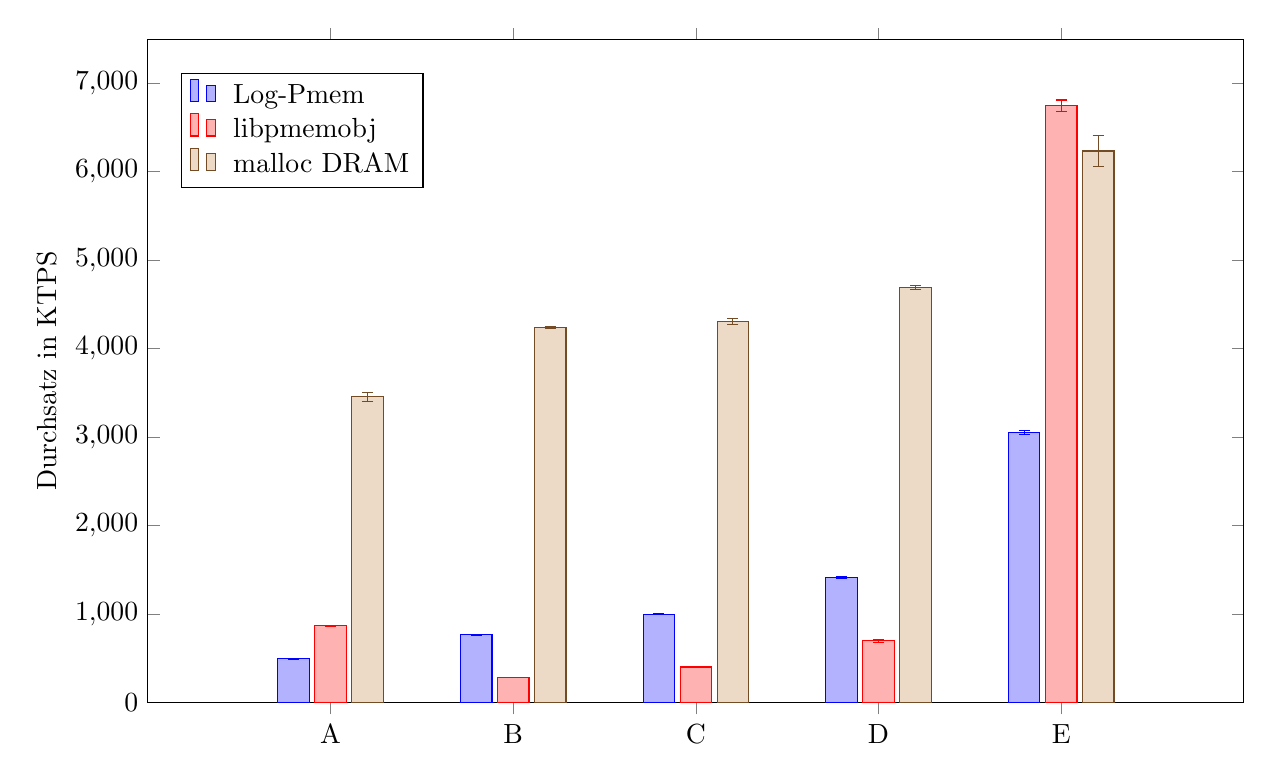
\begin{tikzpicture}
			\begin{axis} [
				ybar,
				height=10cm,
				width=15.5cm,
				bar width=0.4cm,
				major grid style={draw=white},
				ymin=0,
				xtick=data,
				symbolic x coords={A, B, C, D, E},
				enlarge x limits={0.25},
				ylabel=Durchsatz in KTPS,
				legend cell align=left,
				legend style={
					at={(0.03, 0.95)},
					anchor=north west,
					column sep=1ex
				}
				]
				\addplot+ [
				error bars/.cd,
				y dir=both,
				y explicit,
				] coordinates{
					(A, 495.288) +- (0, 3.261190379)
					(B, 767.131) +- (0, 6.486498251)
					(C, 997.326) +- (0, 7.029569162)
					(D, 1411.381) +- (0, 7.961850853)
					(E, 3053.630) +- (0, 20.9351685)
				};
				
				\addplot+ [
				error bars/.cd,
				y dir=both,
				y explicit,
				]  coordinates{
					(A, 868.227) +- (0, 5.875680488)
					(B, 285.616) +- (0, 1.907582252)
					(C, 401.952) +- (0, 3.021553839)
					(D, 697.423) +- (0, 13.53687363)
					(E, 6742.447) +- (0, 63.37766768)
				};
				
				\addplot+ [
				error bars/.cd,
				y dir=both,
				y explicit,
				]  coordinates{
					(A, 3455.150) +- (0, 51.968)
					(B, 4236.384) +- (0, 12.69304865)
					(C, 4307.213) +- (0, 35.05238453)
					(D, 4689.690) +- (0, 23.72500242)
					(E, 6229.567) +- (0, 179.3222963)
				};
				
				\legend {Log-Pmem, libpmemobj, malloc DRAM};
			\end{axis}
		\end{tikzpicture}
		\caption{Durchschnittlicher Durchsatz in Tausend Transaktionen pro Sekunde für Log-strukturierten Heap, libpmemobj und malloc für die Workloads A bis E}
		\label{ergebnisseDiagramm}
	\end{figure}
	
	\begin{table}[H]
		\begin{center}
			\begin{tabular}{c | c | c | c | c | c}
				& Workload A & Workload B & Workload C & Workload D & Workload E \\ \hline
				Log-Pmem & 495,288 & 767,131 & 997,326 & 1411,381 & 3053,630 \\
				libpmemobj & 868,227 & 285,616 & 401,952 & 697,423 & 6742,447 \\
				malloc DRAM & 3455,150 & 4236,384 & 4307,213 & 4689,690 & 6229,567
			\end{tabular}
		\end{center}
		\caption{Durchschnittlicher Durchsatz in Tausend Transaktionen pro Sekunde für Log-strukturierten Heap, libpmemobj und malloc für die Workloads A bis E}
		\label{ergebnisseTabelle}
	\end{table}
	
	Wie zu erwarten war ist DRAM schneller als NVRAM, das gilt überraschenderweise jedoch nicht für Workload E, denn hier hat libpmemobj einen besseren Durchsatz. 
	Workload E besteht nur aus Lesezugriffen, um diese im Benchmark darzustellen, wird ein Pointer als Argument übergeben an dessen Stelle die Adresse der Daten geschrieben wird.
	Bei dem Benchmark für DRAM ist das also nur eine einzige Anweisung, welche die Adresse setzt.
	Bei libpmemobj kommt zusätzlich noch die Umwandlung des Typs \code{PMEMoid} dazu, das ist das gleiche Prinzip wie die Offsets beim Log-strukturierten Heap, bevor die Adresse gesetzt wird. Hier sind es also zwei Anweisungen.
	Trotzdem ist der Benchmark für libpmemobj hier schneller, auch nach mehrmaligem wiederholen beider Benchmarks ändert sich das nicht.
	Warum genau das passiert, ist nicht klar und kann hier nur spekuliert werden.
	
	An den Ergebnissen lässt sich gut erkennen, wann der Log-strukturierte Heap schneller und langsamer ist als libpmemobj, bzw. allgemeiner wann eine Log-Struktur besser und schlechter ist als ein general-purpose Allokator.
	In den Workloads B, C und D hat der Log-strukturierte Heap mehr als doppelt so viel Durchsatz wie libpmemobj. 
	Bei Workloads A und E ist es anders herum, wobei es bei Workload A nicht ganz das Doppelte ist.
	Wenn man sich die Workloads noch einmal anschaut, ist das auch logisch so.
	
	Zuerst zu Workload E: libpmemobj gibt bei einer Allokation zwar nicht, wie malloc, direkt die Adresse zurück, aber einen Typ der sich einfach zu der Adresse konvertieren lässt, da sich hier die Daten im NVRAM immer an der selben Stelle befinden.
	Beim Log-strukturierten Heap muss die tatsächliche Adresse immer erst angefragt werden, da sie sich ständig ändern kann.
	Durch dieses Abfragen kommt ein nicht einmal halb so großer Durchsatz zu Stande.
	
	Die Workloads B, C und D fügen zusätzlich Daten ein. Die Verhältnisse zwischen Lesen und Einfügen sind: für B 25/75, für C 50/50 und für D 75/25.
	Die große Stärke des Log-strukturierten Heaps ist das Allozieren von Speicher. Denn es muss nicht erst eine freie Stelle im Speicher gefunden werden, an der die Daten abgelegt werden können.
	Es steht von Anfang an fest, wo neue Daten gespeichert werden, am Ende des Logs. 
	General-purpose Allokatoren, wie libpmemobj müssen immer erst eine passende freie Stelle im Speicher finden.
	Das kostet, wie die Ergenisse zeigen, deutlich mehr Zeit. Und zwar soviel, dass selbst bei Workload D, der zu 75 Prozent liest und nur zu 25 Prozent alloziert, der Log-strukturierte Heap mehr als doppelt so schnell ist, obwohl er deutlich langsamer liest, wie Workload E zeigt.
	
	Workload A liest gar nicht, fügt aber auch nur zu 10 Prozent neue Daten ein, die restlichen 90 Prozent der Zeit werden bestehende Daten aktualisiert. Auch hier ist wieder logisch zu erklären warum libpmemobj fast doppelt so viel Durchsatz hat.
	Wie bereits erwähnt befinden sich die allozierten Daten bei libpmemobj immer an der selben Stelle, daher kann nicht nur beim lesen direkt die Adresse verwendet werden, sondern auch beim aktualisieren können die neuen Daten direkt an die Adresse geschrieben werden.
	Beim Log-strukturierten Heap ist das nicht erlaubt, da Daten im Log nicht verändert werden dürfen.
	Es wird stattdessen jedes mal ein neuer Eintrag in das Log eingefügt, was langsamer ist als die Daten direkt in den Speicher zu schreiben.
%	\\
%	\\
%	Welcher Allokator schneller ist, hängt also vom Anwendungsfall ab. Der Log-strukturierte Heap kann schneller schreiben, während libpmemobj ohne Transaktionen schneller lesen und Daten aktualisieren kann.
	
	
	
	\section{Hashtabelle persistieren und rekonstruieren}
	
	Um zu prüfen, ob es sich überhaupt lohnt die Hashtabelle zu persistieren, anstatt sie einfach jedes mal aus den bestehenden Daten zu rekonstruieren, wurde für beide Optionen die benötigte Zeit für zwei verschiedene Szenarien gemessen. 
	Dabei wurde der Cleaner ausgeschaltet, um jedes mal die selben Daten zu haben. 
	Jeder Test wurde fünf mal ausgeführt.

	Im ersten Test beinhaltet der Speicher zwei Millionen Strings mit einer zufälligen Länge von bis 1024 Zeichen.
	Die persistierte Hashtabelle zu laden dauerte im Schnitt 0,1615532 Sekunden. Sie zu rekonstruieren 0,7058198 Sekunden.
	Die Hashtabelle zu persistieren und laden ist um ein Vielfaches schneller, bei dieser Menge an Daten dauert jedoch beides nicht lange.
	
	Im zweiten Test befinden sich zehn Millionen Strings mit einer Länge von zwölf Zeichen im Speicher.
	Hier dauerte das Laden im Durchschnitt 8,5754988 Sekunden und das Rekonstruieren 0,4172964 Sekunden.
	
	Bei vielen kleinen Daten ist das Rekonstruieren der Hashtabelle also definitiv die bessere Option.
	Bei größeren Daten ist es schneller die Hashtabelle zu persistieren und zu laden.
	
	
	
	\chapter{Zusammenfassung und Ausblick}
	
	\section{Zusammenfassung}
	
	In dieser Arbeit wurde ein Log-strukturierter Heap für NVRAM entwickelt. Dafür werden neben dem Log noch eine Hashtabelle und ein Cleaner benötigt.
	Auch an potenziell entstehende Probleme durch Abstürze wurde gedacht, sodass entsprechende Maßnahmen eingeleitet werden, um Datenverlust zu verhindern und den Speicher konsistent zu halten.
	Für die Implementierung wurden die Bibliotheken libpmem2 des PMDKs \cite{PMDK:Docs}, für alles was mit dem Arbeiten auf NVRAM in Verbindung steht, sowie GLib \cite{GLib} für die Verwendung als Hashtabelle und des Testingframeworks verwendet.
	
	Zum evaluieren der Arbeit wurde der bestehende Benchmark pmemids\_bench \cite{Bench:Git} verwendet, in welchen die Arbeit leicht eingebunden werden konnte. Verglichen wurde die Implementierung mit malloc, dem Standard C Allokator für DRAM, und libpmemobj ohne Transaktionen \cite{PMDK:Docs}, einem general-purpose Allokator für NVRAM.
	Die Ergebnisse waren bis auf eine kleine Ausnahme, die nicht die Implementierung dieser Arbeit betrifft, so erwartbar. Sie zeigen, dass das Arbeiten auf DRAM, bis auf eine Ausnahme, schneller ist, als auf NVRAM.
	Außerdem zeigen sie die Vor- und Nachteile eines Log-strukturierten Heaps gegenüber eines general-purpose Allokators. 
	Welche speziell für die Implementierung dieser Arbeit sind, dass bei einer Log-Struktur mehr als doppelt so schnell Speicher alloziert, dafür aber nur halb so langsam gelesen und fast, fast halb so langsam aktualisiert werden kann.
	
	
	
	\section{Ausblick}
	
	Aktuell läuft der Cleaner schon mit mehreren Threads, der Allokator selbst aber nicht. Das bedeutet auch, das immer nur ein Programm gleichzeitig auf die Datei im NVRAM zugreifen darf, welche das Log enthält. Hier besteht die Möglichkeit die Implementierung so umzubauen, dass mehrere Threads gleichzeitig Speicher allozieren können. 
	Außerdem wäre es schön, wenn eine bessere Synchronisierung der Cleanerthreads umgesetzt wird, bei der weniger Abschnitte gelockt werden müssen und somit mehr Parallelität möglich ist.
	Ebenfalls den Cleaner betreffend, könnte durch Experimente optimiert werden, wann sich dieser dafür entscheidet ein Segment zu säubern bzw. allgemein überhaupt das Log zu säubert. Aktuell liegt die Grenze jeweils bei fünfzig Prozent belegtem Speicher.
	Zuletzt könnte eine bessere Cleaningstrategie entwickelt werden. Momentan werden noch aktive Daten vom Cleaner in der Reihenfolge umkopiert, in der er sie vorfindet. Stattdessen könnte der Cleaner diese sortieren und gruppieren, um eine bessere Performance zu erreichen. 
	Z.B. Einträge, die häufig bzw. selten aktualisiert werden zusammen.




  \end{thesis}

\end{document}

